\documentclass{beamer}
\usetheme{Berlin}
\usepackage[latin1]{inputenc}
\usepackage{graphicx}
\usepackage{alltt}
\usepackage[spanish]{babel}
\title{Informe de Tarea 3 - Juego Skynet}
\author{Francisco Ar\'evalo\\
  \texttt{francisco.arevalod@alumnos.usm.cl}\\
  \texttt{http://github.com/farevalod/fisw-tarea3}\\
  \vspace{10mm}
  Departamento de Inform\'atica\\
  Universidad T\'ecnica Federico Santa Mar\'ia\\
  Santiago, Chile}
\date{\today}
\begin{document}
\maketitle
\section{Class diagram}
\begin{frame}
Jugador is a bridge between Usuario and Robot.\\
Game area is defined by setting an upper-left corner, a height and a width.\\
Events between players and robots are logged, recording coordinates, timestamp, and details of the interaction.\\
Users can set up teams and share items, and check their scores at any time.
\begin{figure}[htb]
\centering
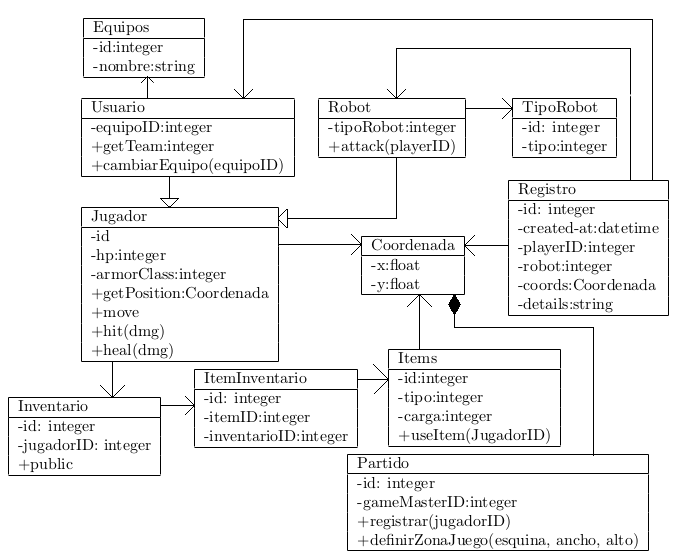
\includegraphics[scale=0.3]{clases}
\caption{Class Diagram}
\end{figure}
\end{frame}
\section{Interaction Diagrams}
\begin{frame}
\subsection{User/Robot interaction}
User can use an Item to attack a robot. The damage inflicted will depend on a calculation considering AC, range, and item damage.
User can use Items to heal, or improve his AC.
Robots can attack Users. If the user's HP drops below 0, he is removed from the map.
If the robot is disabled, the user earns points depending on robot type.
\begin{figure}[htb]
\centering
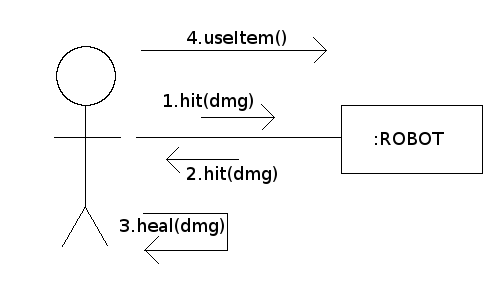
\includegraphics[scale=0.4]{user-robot}
\caption{User/Robot interaction}
\end{figure}
\end{frame}
\begin{frame}
\subsection{User/Item interaction}
Users can collect, share, and use items they find on the map. When an user picks up an item, it is stored in his inventory. Depending on the type of item, the user can heal himself, load a weapon with ammo, improve his Armor Class, or use the item to attack a robot. Items have a charge level that shows number of times the item can be used. Users can share items with their teams if they choose to do so, via the Item menu.
\begin{figure}[htb]
\centering
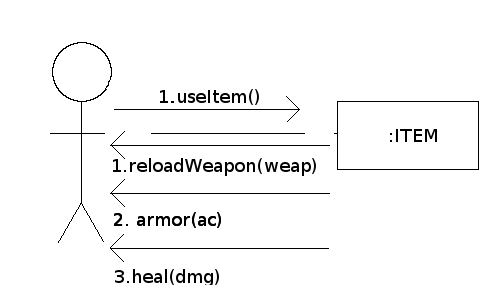
\includegraphics[scale=0.4]{item}
\caption{User/Item interaction}
\end{figure}
\end{frame}
\begin{frame}
\section{User Interfaces}
This is the main game screen. The device's camera is activated, and an overlay is shown over the picture, detailing HUD data (HP, armor, remaining ammo on weapon), a button to access the item menu, and a map showing robots, players and items. Robots are shown in an augmented reality view. The user can access a main menu via a physical button.
\subsection{Heads Up Display}
\begin{figure}[htb]
\centering
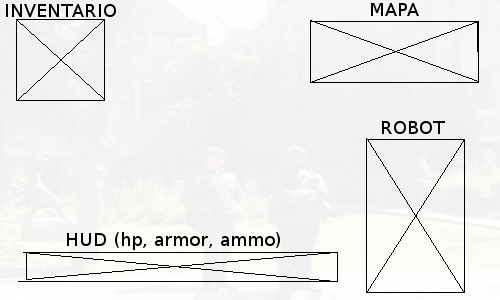
\includegraphics[scale=0.5]{hud}
\caption{Heads Up Display}
\end{figure}
\end{frame}
\begin{frame}
\subsection{Item Menu}
The player can use this menu to check his inventory, and select an item for use. Information regarding the item, such as effects and current charge, will be shown on the screen. The user can cycle through his items, and items shared by his team.
\begin{figure}[htb]
\centering
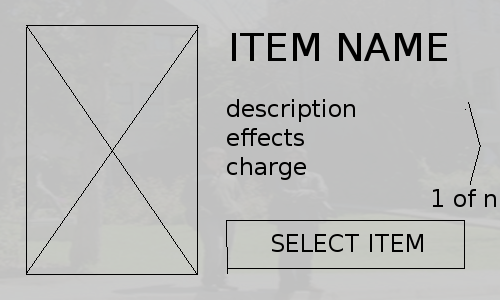
\includegraphics[scale=0.5]{item-menu}
\caption{Item Menu}
\end{figure}
\end{frame}
\begin{frame}
\subsection{Main Menu}
This menu lets the user configure his player information, such as name and team. A player can surrender at any time by selecting the "Leave Game" option. Players can check their scores, and compare against a leaderboard. There is an option to report abuse or game issues to a Game Master.
\begin{figure}[htb]
\centering
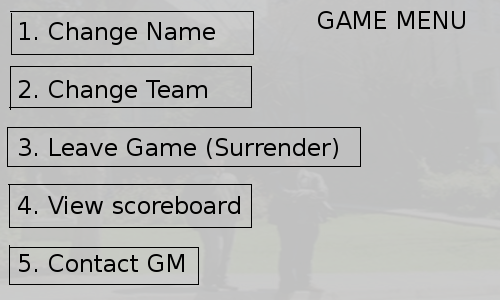
\includegraphics[scale=0.5]{main-menu}
\caption{Main Menu}
\end{figure}
\end{frame}
\end{document}
